% begin module polar-curve-ex4
\begin{frame}
\begin{example}[Example 4, p. 677]
What curve is represented by the polar equation $r = 2$?
\begin{columns}[c]
\column{.5\textwidth}
\ \only<handout:0| -2>{%
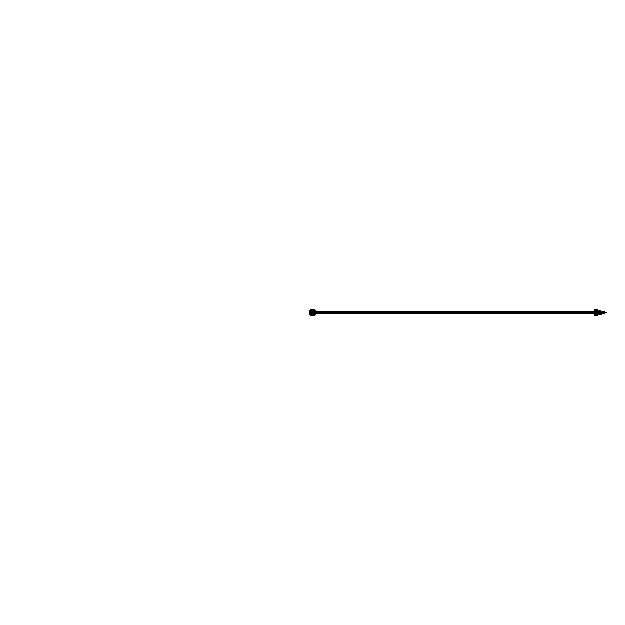
\includegraphics[height=6cm]{polar-curves/pictures/11-03-ex4a.pdf}%
}%
\only<handout:0| 3>{%
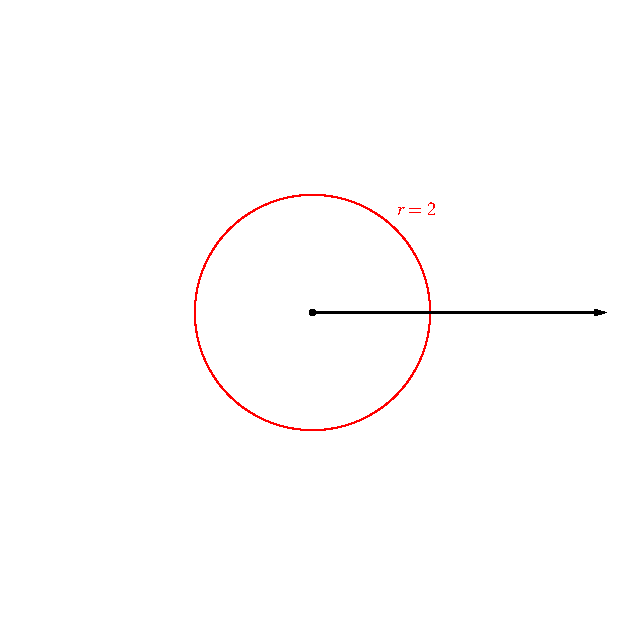
\includegraphics[height=6cm]{polar-curves/pictures/11-03-ex4b.pdf}%
}%
\only<handout:0| 4>{%
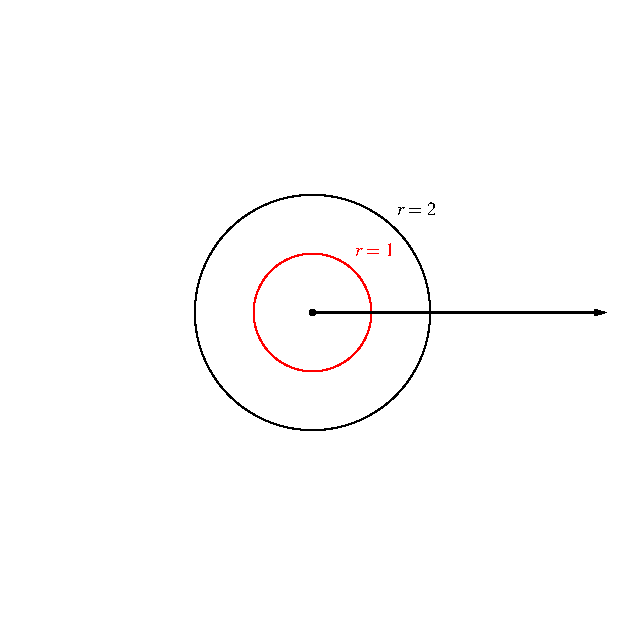
\includegraphics[height=6cm]{polar-curves/pictures/11-03-ex4c.pdf}%
}%
\only<5->{%
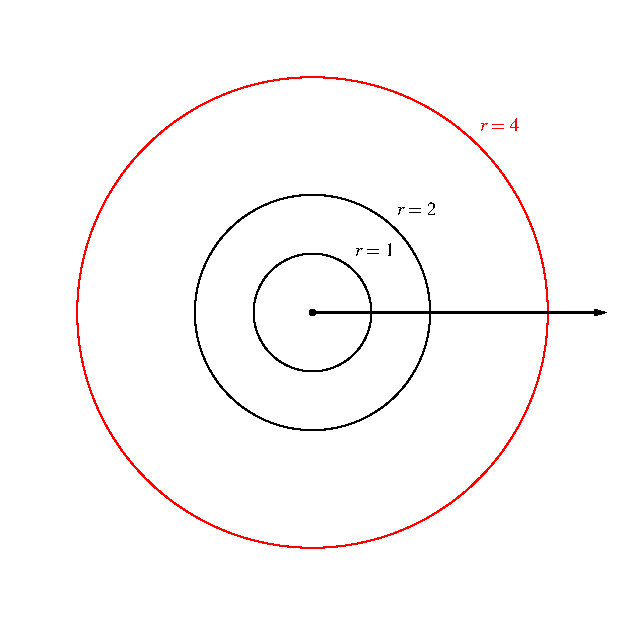
\includegraphics[height=6cm]{polar-curves/pictures/11-03-ex4d.pdf}%
}%
\column{.5\textwidth}
\begin{itemize}
\item<2->  The equation describes all points that are $2$ units away from $O$.
\item<3->  This is the circle with center $O$ and radius $2$.
\item<4->  The equation $r = 1$ describes the unit circle.
\item<5->  The equation $r = 4$ describes the circle with center $O$ and radius $4$.
\end{itemize}
\end{columns}
\end{example}
\end{frame}
% end module polar-curve-ex4
